\begin{figure}[!h]
	\begin{minipage}[t]{0.49\linewidth}
		\centering
		\centerline{ 
\includegraphics[width=\linewidth]{motionx} }
		\centerline{(а) Карта амплитуды}
		\centerline{горизонтального движения}\medskip
	\end{minipage}%
	\hfill
	\begin{minipage}[t]{0.49\linewidth}
		\centering
		\centerline{
\includegraphics[width=\linewidth]{motiony} }
		\centerline{(б) Карта амплитуды}
		\centerline{вертикального движения}\medskip
	\end{minipage}
	\begin{minipage}[t]{0.49\linewidth}
		\centering
		\centerline{ 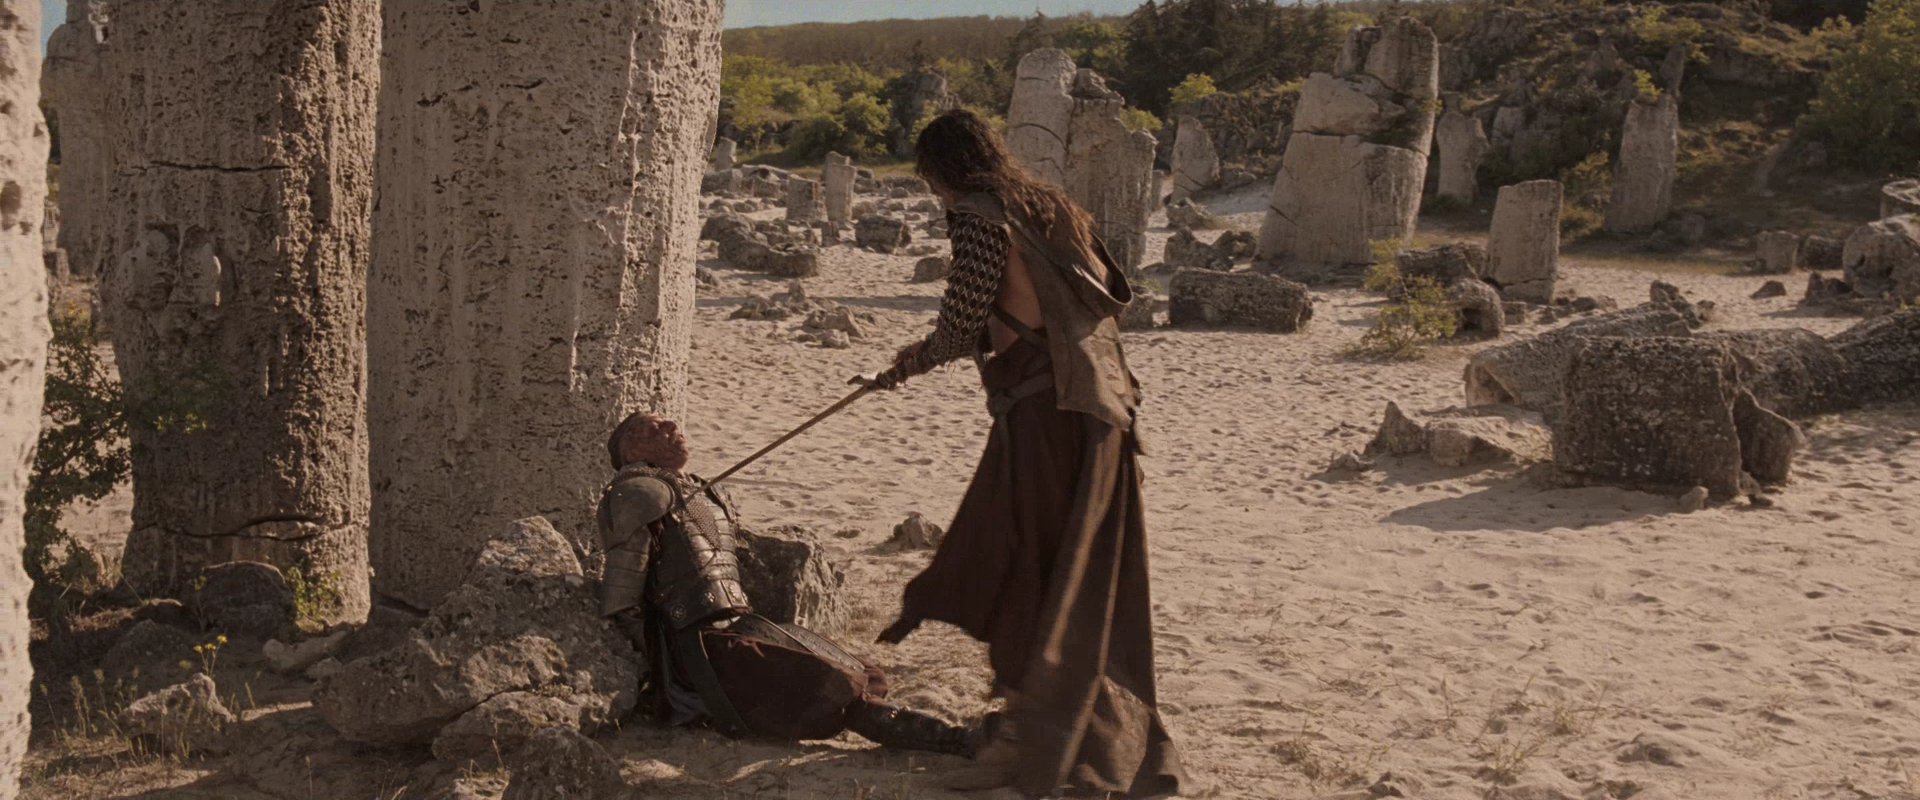
\includegraphics[width=\linewidth]{src} }
		\centerline{(в) Исходный левый ракурс}\medskip
	\end{minipage}%
	\hfill
	\begin{minipage}[t]{0.49\linewidth}
		\centering
		\centerline{
\includegraphics[width=\linewidth]{merged} }
		\centerline{(г) Совмещенная карта}
		\centerline{амплитуды движения}\medskip
	\end{minipage}
	\begin{minipage}[t]{\linewidth}
	\caption{Пример карт горизонтального~(а) и вертикального~(б) движения, извлеченные
        с помощью блочного алгоритма оценки движения~\cite{simonyan2008fast} для левого ракурса исходного кадра~(в).
        Результаты объединяются в одну общую карту амлитуды движения~(г).}
    \label{fig:merged}
    \end{minipage}
\end{figure}
